% MINIPAGE ENV

\begin{minipage}[t]{0.45\linewidth}

\end{minipage}
\hfill
\begin{minipage}[t]{0.45\linewidth}

\end{minipage}

% PRETTY TABLES

\newcolumntype{L}[1]{>{\raggedright\let\newline\\\arraybackslash\hspace{0pt}}m{#1}} % beautiful column types
\newcolumntype{C}[1]{>{\centering\let\newline\\\arraybackslash\hspace{0pt}}m{#1}}

% EXPEX EXAMPLE

\ex\label{ex:}
\begingl
	\gla //
	\glb //
	\glft `' //
\endgl
\xe

\ex\label{ex:}
    \begin{multicols}{2}
    \begin{compactitem}[{}]
    	\item 
    \end{compactitem}
    \end{multicols}
\xe	

%STRICT CV REPRESENTATIONS

			\ex\label{ex:}Example\\
						\emph{gam} $+$ \emph{a} \\
				\begin{tikzpicture}[>=latex]
\matrix [matrix of nodes, row sep=0.1em,
column sep={1.5em,between origins}]
{
|(c1)|{C} & |(v1)|{V} & |(c2)|{C} & |(v2)|{V} & |(c3)|{C} & |(v3)|{V} \\[0.6em]
|(C1)|{g} & |(V1)|{a} & |(C2)|{m} & |(V2)|{ } & |(C3)|{ } & |(V3)|{a} \\
};
\draw (c1.south) -- (C1.north);
\draw (v1.south) -- (V1.north);
\draw (c2.south) -- (C2.north);
\draw (v3.south) -- (V3.north);  % association lines
\draw [->] (v3.north) -- ++(north:2.5ex) -| (v2.north) node[midway,above right] {G};  % government arrow
\draw [->] (v2.120) -- ++(north:2.5ex) -| (v1.north) node[midway,above right]  {no G} node[pos=0.3,sloped,rotate=45]{$|$}node[pos=0.3,sloped,rotate=45]{$|$};  % crossed-out government arrow
    \scoped[on background layer]  % shading
    {
\node[fill=pink!50, fit=(v2)(c3) ]   {};
    }
				\end{tikzpicture}
			\xe

% TIKZ TREE

% regular

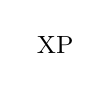
\begin{tikzpicture}[font=\small, level distance=1.7em,
level/.style={sibling distance=3em}]
									
\node {XP};

\end{tikzpicture}

% nanosyntax

\begin{tikzpicture}[level distance=2em, 
			sibling distance=3.7em,
  leaf/.style={
  	isosceles triangle,
	draw,
	isosceles triangle stretches=true, 
	minimum height=1.77em,
	minimum width=1em,
	shape border rotate=90,
	yshift={0mm},font=\tiny}]
\node (tree) 
	{\textsc{}}
	child {node {\textsc{}} child {node[leaf] { }}}
	child {node (i) {\textsc{}}
		child {node {\textsc{}}}};
\node [right= 2 em of tree] {$\Rightarrow$ \textit{WORD}};
\end{tikzpicture}

% TABLE

% regular

\begin{table}[h]
\centering
\begin{tabular}{L{0.6cm}C{1cm}C{1.2cm}}
\toprule
\textbf{}
&
\textbf{}
&
\textbf{}
\\
\midrule
\textbf{}&		&		\\
\addlinespace[0.2cm]
\textbf{}&		&		\\
\addlinespace[0.2cm]
\textbf{}&		&		\\
\bottomrule
\end{tabular}
\caption{}
\label{paragr}
\end{table}

% nanosyntax

\begin{table}[H]
\centering
\begin{tabular}{c c c c c c c c c c c c}
\toprule
\textsc{}&\textsc{xNP}&\textsc{ref}&\textsc{class}&\textsc{fem}&\textsc{ind}&\textsc{f1}&\textsc{f2}&\textsc{f3}&\textsc{f4}&\textsc{f5}&\textsc{f6}\\
\midrule
\textsc{nom}&\multicolumn{2}{|c|}{\cellcolor{gray!70}gub}&\multicolumn{4}{c}{\cellcolor{gray!30}a}&&&&&\\
\textsc{acc}&\multicolumn{2}{|c|}{\cellcolor{gray!70}gub}&\multicolumn{5}{c}{\cellcolor{gray!30}u}&&&&\\
\textsc{gen}&\multicolumn{2}{|c|}{\cellcolor{gray!70}gub}&\multicolumn{6}{c}{\cellcolor{gray!30}y}&&&\\
\textsc{loc}&\multicolumn{2}{|c|}{\cellcolor{gray!70}gub}&\multicolumn{7}{c}{\cellcolor{gray!30}e}&&\\
\textsc{dat}&\multicolumn{2}{|c|}{\cellcolor{gray!70}gub}&\multicolumn{8}{c}{\cellcolor{gray!30}e}&\\
\textsc{ins}&\multicolumn{2}{|c|}{\cellcolor{gray!70}gub}&\multicolumn{9}{c}{\cellcolor{gray!30}oj}\\
\midrule
\textsc{nom}&\multicolumn{6}{|c|}{\cellcolor{gray!70}tetrad'}&&&&&\\
\textsc{acc}&\multicolumn{7}{|c|}{\cellcolor{gray!70}tetrad'}&&&&\\
\textsc{gen}&\multicolumn{3}{|c|}{\cellcolor{gray!70}tetrad'}&\multicolumn{5}{c}{\cellcolor{gray!30}i}&&&\\
\textsc{loc}&\multicolumn{3}{|c|}{\cellcolor{gray!70}tetrad'}&\multicolumn{6}{c}{\cellcolor{gray!30}i}&&\\
\textsc{dat}&\multicolumn{3}{|c|}{\cellcolor{gray!70}tetrad'}&\multicolumn{7}{c}{\cellcolor{gray!30}i}&\\
\textsc{ins}&\multicolumn{3}{|c|}{\cellcolor{gray!70}tetrad'}&\multicolumn{8}{c}{\cellcolor{gray!30}ju}\\
\bottomrule
\end{tabular}
\caption{Lexicalisation table.}
\label{tab:iifem}
\end{table}

% TINY BIBLIOGRAPHY

\usepackage{pifont}

\renewbibmacro*{byeditor+others}{%
  \setunit{\addcomma\space}%
  \ifnameundef{editor}
    {}
    {\usebibmacro{byeditor+othersstrg}%
     \setunit{\addspace}%
     \printnames[byeditor][1-1]{editor}%
     \clearname{editor}%
     \newunit}%
  \usebibmacro{byeditorx}%
  \usebibmacro{bytranslator+others}}
\addbibresource{ref.bib}

\defbibenvironment{bibliography}
  {\noindent}% or {} if you like indentation
  {\unspace}
  {\quad\ding{118}\linespread{.55}\printtext\addspace}

\renewcommand*{\bibfont}{\small\linespread{.55}}

% DRAWING ARROWS IN EXAMPLES

% preamble

\usetikzlibrary{matrix}
\usetikzlibrary{positioning}
\usetikzlibrary{decorations.shapes}
\usetikzlibrary{arrows}
\usetikzlibrary{arrows.meta}
\usetikzlibrary{svg.path}

\DeclareDocumentCommand \tikzexsetup {} {%
\tikzstyle{every picture}+=[remember picture, inner sep=0pt,
                                 baseline, anchor=base]}
% arg 1: optional strut; arg 2: node name; arg 3: node content 
\DeclareDocumentCommand \ND {s m m} {%
\tikzifinpicture{}{\tikz}\node(#2){\IfBooleanTF{#1}{\strut}{}#3};}
\tikzset{exarrows/.style={semithick,
                             arrows={-Stealth[scale=1, scale length=1,
                                              scale width=1]}}}
\definelingstyle{exarrbelow}{belowexskip=1em plus 0.375em minus 0.25em}
\setbeamertemplate{section in toc}{%
    *  \inserttocsection \par}
    
% usage    
    
\pex[lingstyle=exarrbelow, interpartskip=1em plus 0.125em minus 0.125em]
	\a\tikzexsetup%
\ND*{a1}{T\textsuperscript{$\phi$}} {[} -əma\textsuperscript{$\phi$} {[} V \ND*{a2}{NP\textsuperscript{[PL]}} {]} {]} 
	\a\tikzexsetup%
*\ND*{b1}{T\textsuperscript{$\phi$}} {[} -əma\textsuperscript{$\phi$} {[} V \ND*{b2}{NP\textsuperscript{[PART]}} {]} {]} 
	\begin{tikzpicture}[overlay]
     \draw[exarrows] (a1.south) -- ++(south:1.5ex) -| (a2.south);
     \draw[exarrows] (b1.south) -- ++(south:1.5ex) -| (b2.south);
  	\end{tikzpicture}
\xe